
%(BEGIN_QUESTION)
% Copyright 2015, Tony R. Kuphaldt, released under the Creative Commons Attribution License (v 1.0)
% This means you may do almost anything with this work of mine, so long as you give me proper credit

This three-phase transformer configuration is called a Wye-Zigzag:

$$\includegraphics[width=15.5cm]{i00837x01.eps}$$

Calculate the magnitude and phase angle of $V_{X1}$ assuming $V_{H1}$ is 7.2 kV $\angle$ 0$^{o}$ and the phase rotation is H1-H2-H3.

\vskip 10pt

$V_{X1}$ = \underbar{\hskip 50pt}

\vfil 

\underbar{file i00837}
\eject
%(END_QUESTION)





%(BEGIN_ANSWER)

This is a graded question -- no answers or hints given!

%(END_ANSWER)





%(BEGIN_NOTES)

If $V_{H1}$ = 7200 volts $\angle$ 0$^{o}$, and the rotation is H1-H2-H3, then the primary phase voltages must be:

\begin{itemize}
\item{} $V_{H1}$ = 7200 V $\angle$ $0^{o}$
\item{} $V_{H2}$ = 7200 V $\angle$ $-120^{o}$
\item{} $V_{H3}$ = 7200 V $\angle$ $-240^{o}$
\end{itemize}

The 4500:250 turns ratio (18:1) from each primary winding to each secondary winding yields secondary winding voltages of 400 volts each.  At this point it becomes useful to mark the schematic with + and $-$ polarity symbols (as though we were analyzing a DC circuit) with the known voltages:

$$\includegraphics[width=15.5cm]{i00837x02.eps}$$

Note how all the secondary winding voltages bear the same angle as their respective primary winding voltages, because we are working on the assumption that there is negligible phase shift inherent to the transformer.  Note also how all of our + and $-$ polarity marks follow the same pattern as the ``square'' polarity markings on the transformer windings: every ``polarity'' terminal is positive while every ``nonpolarity'' terminal is negative.

\vskip 10pt

At this point we may simply add up the winding pair voltages for each secondary line, respecting polarity as we go:

\begin{itemize}
\item{} $V_{X1}$ = (400 V $\angle$ $-120^{o}$) $-$ (400 V $\angle$ $0^{o}$) = 692.8 V $\angle$ $-150^{o}$
\item{} $V_{X2}$ = (400 V $\angle$ $-240^{o}$) $-$ (400 V $\angle$ $-120^{o}$) = 692.8 V $\angle$ $90^o$
\item{} $V_{X3}$ = (400 V $\angle$ $0^{o}$) $-$ (400 V $\angle$ $-240^{o}$) = 692.8 V $\angle$ $-30^o$
\end{itemize}

\filbreak

The phasor diagram showing secondary winding voltages makes it clear why this is called a ``zigzag'' configuration.  The arrowheads on each winding voltage phasor shows the subtraction at work, with phasor tips meeting at each vertex in the ``zigzag'' shape:

$$\includegraphics[width=15.5cm]{i00837x03.eps}$$

The resultant phasors $V_{X1}$, $V_{X2}$, and $V_{X3}$ are shown in green, while the secondary winding phasors are shown in blue.

%INDEX% Electronics review, 3-phase transformer bank phase shift calculations

%(END_NOTES)

